\documentclass[../mathNotesPreamble]{subfiles}
\begin{document}
%\relscale{1.4} %TODO
\section{16.5: Triple Integrals in Cylindrical and Spherical Coordinates}

  \textbf{Cylindrical coordinates:}\newline
  The concept of polar coordinates in $\bbr^2$ from section 16.3 can be extended to $\bbr^3$. This coordinate system is called \textit{cylindrical coordinates} where every point $P$ in $\bbr^3$ has coordinates $(r,\theta, z)$, where $0\leq r<\infty$, $0\leq\theta\leq 2\pi$, and $-\infty<z<\infty$.

  \begin{thmBox*}[Transformations between Cylindrical and Rectangular Coordinates]
    \vspace*{0.5\baselineskip}
    \begin{minipage}{0.5\linewidth}
      \begin{center}
        \textbf{Rectangular} $\rightarrow$ \textbf{Cylindrical}
      \end{center}
      \begin{align*}
        r^2&=x^2+y^2\\
        \tan\theta&=y/x\\
        z&=z
      \end{align*}
    \end{minipage}%
    \begin{minipage}{0.5\linewidth}
      \begin{center}
        \textbf{Cylindrical} $\rightarrow$ \textbf{Rectangular}
      \end{center}
      \begin{align*}
        x&=r\cos\theta\\
        y&=r\sin\theta\\
        z&=z
      \end{align*}
    \end{minipage}%
  \end{thmBox*}

  \begin{ex*}
    Sketch the following sets represented in cylindrical coordinates:
  \end{ex*}
  \begin{tasks}[after-item-skip=\stretch{1}, label=](2)
    \task $\set{(r,\theta,z): r=a}, a>0$
    \task $\set{(r,\theta,z): 0<a\leq r\leq b}$
  \end{tasks}
  \vspace*{\stretch{1}}
  \pagebreak
  
  \begin{tasks}[after-item-skip=\stretch{1}, label=, resume](2)
    \task $\set{(r,\theta,z): z=a}$
    \task $\set{(r,\theta,z): z=ar}, a\neq 0$
    \task $\set{(r,\theta,z): \theta=\theta_0}$
  \end{tasks}
  \vspace*{\stretch{1}}

  \begin{thmBox*}[Theorem 16.6: Change of Variables for Triple Integrals in Cylindrical Coordinates]
    Let $f$ be continuous over the region $D$, expressed in cylindrical coordinates as
      \[D=\set{(r,\theta,z): 0\leq g(\theta)\leq r\leq h(\theta),\ \alpha\leq \theta\leq \beta,\ G(x,y)\leq z\leq H(x,y)}\]
    Then $f$ is integrable over $D$, and the triple integral of $f$ over $D$ is
      \[\iiint\limits_D f(x,y,z)\,dV=\int_\alpha^\beta \int_{g(\theta)}^{h(\theta)}\int_{G\parens{r\cos{\theta},\ r\sin{\theta}}}^{H\parens{r\cos{\theta},\ r\sin{\theta}}}f\parens{r\cos{\theta},\, r\sin{\theta}}\,dz\,r\,dr\,d\theta.\]
  \end{thmBox*}
  \pagebreak

  \begin{ex*}
    Evaluate the following integral using cylindrical coordinates:\newline
      $\displaystyle\int_0^3 \int_0^{\sqrt{9-x^2}} \int_0^{\sqrt{x^2+y^2}} \parens{x^2+y^2}^{-1/2}\,dz\,dy\,dx$
  \end{ex*}
  \vspace*{\stretch{1}} %TODO
  \begin{flushright}
    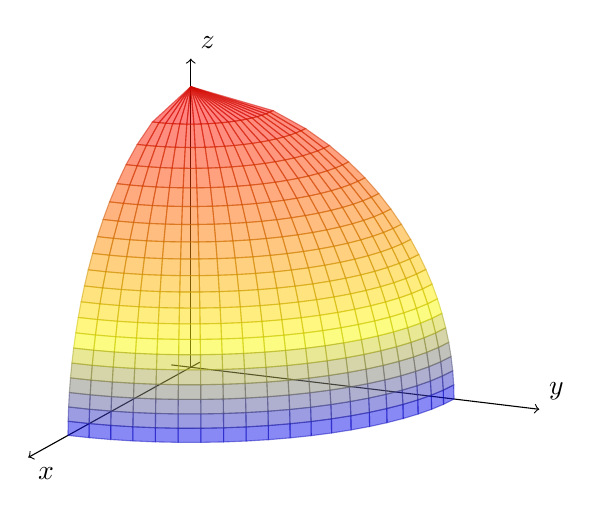
\begin{tikzpicture}
      \begin{axis}[
        axis lines=center,
        axis line style={black,->},
        axis equal,
        xmin=-0,  xmax=1.25,  xmajorticks=false,
        ymin=-0,  ymax=1.25,  ymajorticks=false,
        zmin=0,   zmax=1.10,  zmajorticks=false,
        ticklabel style={font=\normalsize,inner sep=0.5pt,fill=white,opacity=1.0, text opacity=1},
        xlabel=$x$, xlabel style={at={(ticklabel* cs:1)},anchor=north west},
        ylabel=$y$, ylabel style={at={(ticklabel* cs:1)},anchor=south west},
        zlabel=$z$, zlabel style={at={(ticklabel* cs:1)},anchor=south west},
        view={115}{15},
        ]
        \addplot3[surf, opacity = 0.5,
          samples=21,
          domain=0:1,
          y domain=0:0.5*pi,
          z buffer=sort]
          ({sqrt(1-x^2) * cos(deg(y))},
          {sqrt( 1-x^2 ) * sin(deg(y))},
          x);
      \end{axis}
    \end{tikzpicture}
  \end{flushright}
  \pagebreak

  \begin{ex*}
    Find the volume of the solid bounded below by the paraboloid $z=x^2+y^2$ and bounded above by the cone $z=2-\sqrt{x^2+y^2}$.
  \end{ex*}
  \vspace{\stretch{1}} %TODO
  \begin{flushright}
    \begin{tikzpicture}
      \begin{axis}[
        axis lines=center,
        axis line style={black,<->},
        xmin=-1.05,  xmax=1.05,  xmajorticks=false,
        ymin=-1.05,  ymax=1.05,  ymajorticks=false,
        zmin=0,      zmax=2.15,  zmajorticks=false,
        ticklabel style={font=\normalsize,inner sep=0.5pt,fill=white,opacity=1.0, text opacity=1},
        xlabel=$x$, xlabel style={at={(ticklabel* cs:1)},anchor=north west},
        ylabel=$y$, ylabel style={at={(ticklabel* cs:1)},anchor=south west},
        zlabel=$z$, zlabel style={at={(ticklabel* cs:1)},anchor=south west},
        view={105}{27.5},
        ]
        \addplot3 [surf, draw=none, opacity=0.5, restrict z to domain=0:2, data cs=polar, domain=0:360, y domain=0:1] (x, y, y^2);
        \addplot3[domain=0:2*pi, samples=100, samples y=0, -, ClemsonPurple, line width=1pt] ({cos(deg(x))},{sin(deg(x))},1);
        \addplot3 [surf, draw=none, opacity=0.5, restrict z to domain=0:2, data cs=polar, domain=0:360, y domain=0:1] (x, y, 2-y);
      \end{axis}
    \end{tikzpicture}
  \end{flushright}
  \pagebreak

  \textbf{Spherical Coordinates:}\newline
  Spherical coordinates can represent a point $P$ in $\bbr^3$ as $(\rho, \varphi, \theta)$ where
  \begin{itemize}
    \item $\rho$ is the distance from the origin to $P$,
    \item $\varphi$ is the angle between the positive $z$-axis and the line $OP$, and
    \item $\theta$ is the same angle as in cylindrical coordinates.
  \end{itemize}
  \vspace*{\stretch{1}}
  \begin{center}
    \includegraphics[width=0.4\linewidth]{../images/briggs_16_05/fig16_55}
    \hspace*{25pt}
    \includegraphics[width=0.4\linewidth]{../images/briggs_16_05/fig16_56}
  \end{center}
  \vspace*{\stretch{1}}

  \begin{thmBox*}[Transformations between Spherical and Rectangular Coordinates]
    \vspace*{0.5\baselineskip}
    \begin{minipage}{0.5\linewidth}
      \begin{center}
        \textbf{Rectangular} $\rightarrow$ \textbf{Spherical}
      \end{center}
      \begin{align*}
        \rho^2&=x^2+y^2+z^2\\
        &\hspace*{-15pt}\textnormal{Use trigonometry to find}\\
        &\hspace*{-15pt}\varphi \textnormal{ and } \theta.
      \end{align*}
    \end{minipage}%
    \begin{minipage}{0.5\linewidth}
      \begin{center}
        \textbf{Spherical} $\rightarrow$ \textbf{Rectangular}
      \end{center}
      \begin{align*}
        x&=\rho\sin(\varphi)\cos(\theta)\\
        y&=\rho\sin(\varphi)\sin(\theta)\\
        z&=\rho\cos(\varphi)
      \end{align*}
    \end{minipage}%
  \end{thmBox*}

  \pagebreak
  \begin{center}
  %https://tex.stackexchange.com/questions/337570/tabularx-with-different-column-widths
    \renewcommand{\tabularxcolumn}[1]{m{#1}} %sets columns to vertically centered
    \relscale{0.775}
    \begin{tabularx}{\linewidth}{@{}
      >{\hsize=0.575\hsize}X@{\hspace*{20pt}}
      >{\hsize=1.80\hsize}X@{\hspace*{20pt}}
      >{\hsize=0.625\hsize}Y}\toprule
      \textbf{Name}& 
      \textbf{Description}& 
      \textbf{Example}\\\midrule
      %
      Sphere, radius $a$, center $(0,0,0)$&
      $\set{(\rho, \varphi, \theta): \rho=a}, a>0$&
      \includegraphics[width=0.525\linewidth]{../images/briggs_16_05/table16p5_sphere}\\
      %
      Cone&
      $\set{(\rho,\varphi, \theta): \varphi=\varphi_0}, \varphi_0\neq 0, \pi/2, \pi$&
      \includegraphics[width=0.525\linewidth]{../images/briggs_16_05/table16p5_cone}\\
      %
      Vertical\newline half-plane&
      $\set{(\rho,\varphi, \theta): \theta=\theta_0}$&
      \includegraphics[width=0.525\linewidth]{../images/briggs_16_05/table16p5_vertHalfPlane}\\
      %
      Horizontal\newline plane, $z=a$&
      $a>0: \set{(\rho,\varphi, \theta): \rho=a\sec(\varphi),\ 0\leq \varphi< \pi/2}$\newline
      $a<0: \set{(\rho,\varphi, \theta): \rho=a\sec(\varphi),\ \pi/2< \varphi\leq \pi}$&
      \includegraphics[width=0.525\linewidth]{../images/briggs_16_05/table16p5_horizHalfPlane}\\
      %
      Cylinder,\newline radius $a>0$&
      $\set{(\rho,\varphi, \theta): \rho=\alpha\csc(\varphi),\ 0<\varphi<\pi}$&
      \includegraphics[width=0.525\linewidth]{../images/briggs_16_05/table16p5_cylinder}\\
      %
      Sphere,\newline radius $a>0$\newline center $(0,0,a)$&
      $\set{(\rho,\varphi, \theta): \rho=2a\cos(\varphi),\ 0\leq\varphi\leq\pi/2}$&
      \includegraphics[width=0.525\linewidth]{../images/briggs_16_05/table16p5_sphereOffset}\\
      \bottomrule
    \end{tabularx}
  \end{center}
  \pagebreak

  \begin{thmBox*}[Theorem 16.7: Change of Variables for Triple Integrals in Spherical Coordinates]
    Let $f$ be continuous over the region $D$, expressed in spherical coordinates as
      \[D=\set{(\rho,\varphi,\theta): 0\leq g(\varphi,\theta)\leq \rho\leq h(\varphi,\theta),\ a\leq \varphi\leq b,\ \alpha\leq \theta\leq \beta}.\]
    Then $f$ is integrable over $D$, and the triple integral of $f$ over $D$ is
    \begin{align*}
      \mathrlap{\iiint\limits_D f(x,y,z)\,dV}&\\
      &=\int_\alpha^\beta \int_a^b \int_{g(\varphi,\theta)}^{h(\varphi,\theta)}f\parens{\rho\sin(\varphi)\cos(\theta),\,\rho\sin(\varphi)\sin(\theta),\,\rho\cos(\varphi)}\,\rho^2 \sin(\varphi)\ d\rho\,d\varphi\,d\theta.
    \end{align*}
  \end{thmBox*}

  \begin{ex*}
    Evaluate $\iiint\limits_D \parens{x^2+y^2+z^2}\inv[3/2]\,dV$, where $D$ is the region in the first octant between two spheres of radius $1$ and $2$ centered at the origin
  \end{ex*}
  \vspace*{\stretch{1}}
  \pagebreak

  \begin{ex*}
    Find the volume of the solid region $D$ that lies inside the cone $\varphi=\pi/6$ and inside the sphere $\rho=4$.
  \end{ex*}

  \pagebreak
  
\end{document}
